\documentclass[a4paper, 12pt, twocolumn]{ctexart}

\usepackage[top=2cm, bottom=2cm, left=2cm, right=2cm]{geometry}
\usepackage{amsmath}
\usepackage{float}
\usepackage{booktabs}
\usepackage{graphics, graphicx}
\usepackage{fancyhdr}
\pagestyle{fancy}
\renewcommand{\headrulewidth}{0pt}
\fancyhead{}
\usepackage{listings}
\usepackage{xcolor}
\lstset{
	language = c++,
	columns = fixed,
	breaklines = true,
	tabsize = 4,
	frame = single,
	columns = fullflexible,
	commentstyle = \color[RGB]{0,128,0},
	keywordstyle = \color{blue}\bfseries,
	basicstyle   = \small\ttfamily,
	stringstyle  = \color{purple}\ttfamily,
	rulesepcolor = \color{red!20!green!20!blue!20},
	showstringspaces = false
}
\setlength{\columnsep}{20pt}
\setlength{\columnseprule}{0.3pt}

\title{蓝桥历年真题}
\author{}
\date{}

\begin{document}
	\maketitle
	\tableofcontents
	
	\newpage
	\section{2018 C/C++ A组}
	
	\subsection{三角形面积(13分)}
	
	已知三角形三个顶点在直角坐标系下的坐标分别为:$(2.3, 2.5),	(6.4, 3.1),	(5.1, 7.2)$,求该三角形的面积。
	
	注意,要提交的是一个小数形式表示的浮点数。要求精确到小数后3位,如不足3位,需要补零。
	
	\subsection{阅兵方阵(39分)}
	
	$x$国要参加同盟阅兵活动。主办方要求每个加盟国派出的士兵恰好能组成 2 个方阵。$x$国发现弱小的$y$国派出了130人的队伍,他们的士兵在行进中可以变换2种队形:$130 = 81 + 49 = 9^2 + 7^2$、$130 = 121 + 9 = 11^2 + 3^2$

	$x$国君很受刺激,觉得$x$国面积是$y$国的6倍,理应变出更多队形。
	
	于是他发号施令:我们要派出一支队伍,在行进中要变出 12 种队形!!!
	
	手下人可惨了,要忙着计算至少多少人才能组成 12 种不同的双方阵。
	请你利用计算机的优势来计算一下,至少需要多少士兵。
	
	(PS: 不要失去信心,1105人就能组成4种队形了)
	
	注意,需要提交的是一个整数,表示至少需要士兵数目,不要填写任何多余的内容。
	
	
	\subsection{找假币(27分)}
	
	在8枚硬币中,有1枚假币,假币外观与真币一模一样,只是重量略轻或略重一点。
	给你一架天平,要求最多称3次,就找出假币,并且知道它是重一些还是轻一些。
	下面的代码给出一个解决方案,仔细分析逻辑,填写划线位置缺少的代码。
	
	\begin{lstlisting}
#include <stdio.h>
		
int balance(int a, int b) {
	if(a<b) return -1;
	if(a>b) return 1;
	return 0;
}
		
void judge(char* data, int a, int b, int std) {
	switch(balance(data[a],data[std])){
		case -1:
			printf("%d light\n", a);
			break;
		case 0:
			printf("%d heavy\n", b);
			break;
		case 1:
			printf("err!\n", b);
	}
}
		
// data 中8个元素,有一个假币,或轻或重
void f(char* data)	{
	switch( ___________ ){  // 填空
		case -1:
			switch(balance(data[0]+data[4],data[3]+data[1])){
				case -1:
					judge(data,0,3,1);
					break;
				case 0:
					judge(data,2,5,0);
					break;
				case 1:
					judge(data,1,4,0);
			}
			break;
		case 0:
			judge(data,6,7,0);		
			break;
		case 1:
			switch(balance(data[0]+data[4],data[3]+data[1])){
				case -1:
					judge(data,4,1,0);
					break;
				case 0:
					judge(data,5,2,0);
					break;
				case 1:
					judge(data,3,0,1);
			}
			break;		
	}	
}
		
int main() {
	int n, i;
	char buf[100];		
	scanf("%d", &n);
	gets(buf);		
	for(i=0; i<n; i++){
		gets(buf);
		f(buf);
	}		
	return 0;
}
	\end{lstlisting}
	
	请注意:只需要填写划线部分缺少的内容,不要抄写已有的代码或符号。
	
	
	\subsection{约瑟夫环(41分)}
	
	$n$ 个人的编号是 $[1,n]$,如果他们依编号按顺时针排成一个圆圈,从编号是1的人开始顺时针报数。
	(报数是从1报起)当报到 $k$ 的时候,这个人就退出游戏圈。下一个人重新从1开始报数。
	求最后剩下的人的编号。这就是著名的约瑟夫环问题。
	
	本题目就是已知 $n,k$ 的情况下,求最后剩下的人的编号。
	
	题目的输入是一行,2个空格分开的整数$n$, $k$
	要求输出一个整数,表示最后剩下的人的编号。
	
	约定:$0 < n,k < 10^6$
	
	例如输入:
	10 3
	
	程序应该输出:
	4
	
	资源约定:峰值内存消耗(含虚拟机) < 256M,CPU消耗  < 1000ms
	
	
	\subsection{自描述序列(71分)}
	
	小明在研究一个序列,叫Golomb自描述序列,不妨将其记作$\{G(n)\}$。这个序列有2个很有趣的性质:
	
	1. 对于任意正整数$n$,$n$在整个序列中恰好出现$G(n)$次。
	
	2. 这个序列是不下降的。
	
	以下是$\{G(n)\}$的前几项:
	
	n	1	2	3	4	5	6	7	8	9	10	11	12	13
	
	G(n)	1	2	2	3	3	4	4	4	5	5	5	6	6
	
	给定一个整数$n$,你能帮小明算出$G(n)$的值吗?
	
	输入:一个整数$n$。  
	
	对于30\%的数据,$1\leq n\leq 10^6 $
	 
	对于70\%的数据,$1\leq n\leq 10^9$
	
	对于100\%的数据,$1\leq n\leq 2\times10^{15}$  
	
	输出:一个整数$G(n)$
	
	
	【样例输入】
	13
	
	【样例输出】
	6
	
	资源约定:峰值内存消耗(含虚拟机)< 256M,CPU消耗  < 1000ms
	

	
	\subsection{采油(109分)}
	
	LQ公司是世界著名的石油公司,为世界供应优质石油。
	
	最近,LQ公司又在森林里发现了一大片区域的油田,可以在这个油田中开采n个油井。
	
	LQ公司在这$n$个油井之间修建了$n-1$条道路,每条道路连接两个油井,路径中间不会路过任何油井,而且这些道路将所有油井连通。
	
	建立油井的时候需要使用一台大型设备,运输起来非常麻烦,LQ公司准备在其中的一个油井位置建立一个空运站,先将设备空运到空运站,之后每次经过他们建立的道路来运输这个大型设备以建立不同的油井,当油井建立完毕后再从空运站将大型设备运走。
	
	为了减少运输的麻烦,公司要求大型设备在道路上运输的总路程是最短的。
	
	在建立油井和采油的过程中需要花费一些人力,第$i$个油井需要花费$B_i$个人,而一旦油井建成,就需要$S_i$个人一直坚守在油井上进行维护。
	
	当然,如果一个人参与了油井的建设,他可以直接留下来维护油井,或者参与下一个油井的建设,但是在维护油井的人不能再参加后续油井的建设了。
	
	现在LQ公司想知道,大型设备运输的总路径长度最短是多少?在保证总路径长度最短的情况下,LQ公司至少需要花费多少人力才能完成所有油井的建立与维护。
	
	【输入格式】
	
	输入的第一行包含一个整数$n$,表示油井的数量。油井由1到$n$依次标号。
	
	第二行包含$n$个整数,依次表示$B_1, B_2, …, B_n$,相邻的整数之间用一个空格分隔。
	
	第三行包含$n$个整数,依次表示$S_1, S_2, …, S_n$,相邻的整数之间用一个空格分隔。
	
	接下来$n-1$行描述油井之间的道路,其中的第i行包含两个整数$a,b$,用一个空格分隔,表示一条道路的起点为$i+1$、终点为$a$,长度为$b$,道路是双向的,设备可以从任意一端运送到另一端,每条道路都可以经过任意多次。数据保证任意两个油井之间都可以通过道路连接。
	
	【输出格式】输出包含两个整数,用一个空格分隔,表示最优情况下大型设备需要运输的总路程,以及在总路程最短的情况下最少需要花费的人力数量。
	
	【样例输入】
	
	2
	
	10 20
	
	15 15
	
	1 8
	
	【样例输出】
	
	16 30
	
	
	【样例说明】
	
	有两种方案达到最优。
	
	方案一:在油井2建立空运站,先建立油井2,再将大型设备运输到油井1建立油井1,最后将大型设备运回油井2。
	
	方案二:在油井1建立空运站,先将大型设备运输到油井2建立油井2,再将大型设备运送到油井1建立油井1。
	
	【样例输入】
	
	6
	
	3 10 20 7 15 9
	
	2 6 10 4 8 7
	
	1 9
	
	1 2
	
	2 5
	
	3 4
	
	3 7
	
	
	【样例输出】
	
	54 38
	
	【数据规模和约定】
	
	对于20\%的数据:$n$不超过10;
	
	另外20\%的数据:每个油井最多和两个油井之间有道路直接连接;
	
	另外10\%的数据:有$n-1$个油井只有一条道路与其他油井连接;
	
	对于100\%的数据:$n$不超过100000,$B$、$S$、$c$均为不超过10000的正整数。
	
	资源约定:峰值内存消耗(含虚拟机) < 256M,CPU消耗  < 1000ms
	
	\section{2017 C/C++ A组}
	
	
	\subsection{平方十位数(17分)}
	
	由0$\sim$9这10个数字不重复、不遗漏,可以组成很多10位数字。这其中也有很多恰好是平方数(是某个数的平方)。比如:1026753849,就是其中最小的一个平方数。
	
	请你找出其中最大的一个平方数是多少?
	
	注意:你需要提交的是一个10位数字,不要填写任何多余内容。
	
	
	\subsection{生命游戏(43分)}
	
	康威生命游戏是英国数学家约翰·何顿·康威在1970年发明的细胞自动机。 这个游戏在一个无限大的2D网格上进行。
	
	初始时,每个小方格中居住着一个活着或死了的细胞。下一时刻每个细胞的状态都由它周围八个格子的细胞状态决定。
	
	具体来说:
	
	1. 当前细胞为存活状态时,当周围低于2个(不包含2个)存活细胞时, 该细胞变成死亡状态。(模拟生命数量稀少)
	
	2. 当前细胞为存活状态时,当周围有2个或3个存活细胞时, 该细胞保持原样。
	
	3. 当前细胞为存活状态时,当周围有3个以上的存活细胞时,该细胞变成死亡状态。(模拟生命数量过多)
	
	4. 当前细胞为死亡状态时,当周围有3个存活细胞时,该细胞变成存活状态。 (模拟繁殖)
	
	当前代所有细胞同时被以上规则处理后, 可以得到下一代细胞图。按规则继续处理这一代的细胞图,可以得到再下一代的细胞图,周而复始。
	
	例如假设初始是:(X代表活细胞,.代表死细胞)
	
	\begin{lstlisting}
.....
.....
.XXX.
.....
	\end{lstlisting}

	
	下一代会变为:
	\begin{lstlisting}	
.....
..X..
..X..
..X..
.....
	\end{lstlisting}
	
	康威生命游戏中会出现一些有趣的模式。例如稳定不变的模式:
	
	\begin{lstlisting}
....
.XX.
.XX.
....
	\end{lstlisting}
	
	还有会循环的模式:
	\begin{lstlisting}
......      ......       ......
.XX...      .XX...       .XX...
.XX...      .X....       .XX...
...XX.      ....X.       ...XX.
...XX.      ...XX.       ...XX.
......      ......       ......
	\end{lstlisting}
	
	本题中我们要讨论的是一个非常特殊的模式,被称作"Gosper glider gun":
	
	\begin{lstlisting}
......................................
.........................X............
.......................X.X............
.............XX......XX............XX.
............X...X....XX............XX.
.XX........X.....X...XX...............
.XX........X...X.XX....X.X............
...........X.....X.......X............
............X...X.....................
.............XX.......................
......................................
	\end{lstlisting}

	
	假设以上初始状态是第0代,请问第1000000000(十亿)代一共有多少活着的细胞?
	
	注意:我们假定细胞机在无限的2D网格上推演,并非只有题目中画出的那点空间。当然,对于遥远的位置,其初始状态一概为死细胞。
	
	注意:需要提交的是一个整数,不要填写多余内容。
	
	\subsection{表达式计算(25分)}
	
	虽然我们学了许久的程序设计,但对于简单的四则混合运算式,如果让我们完全白手起家地编程来解析,还是有点棘手。
	
	这里,我们简化一下问题,假设只有加法和乘法,并且没有括号来改变优先级。再假设参加运算的都是正整数。
	
	在这么多的限制条件下,表达式的解析似乎简单了许多。下面的代码解决了这个问题。请仔细阅读源码,并填写划线部分缺少的代码。
	
	\begin{lstlisting}
#include <stdio.h>
	
int f3(const char* s,int begin,int end){
	int sum = 0;
	int i;
	for(i = begin; i < end; i++){
		if(s[i] == ' ') continue;
		sum = sum * 10 + (s[i]-'0');
	}
	return sum;
}
	
int f2(const char* s,int begin,int end){
	int p = begin;
	int pro = 1;
	while(1){
		int p0 = p;
		while(p != end && s[p] != '*')
			p++;
		pro *= _________________;  // 填空
		if (p == end) break; 
		p++;
	}
	printf("f2: pro=%d\n", pro);
	return pro;
}
	
int f(const char* s) {
	int p = 0;
	int sum = 0;
	while(1){
		int p0 = p;
		while(s[p]!=0 && s[p]!='+') p++;
		sum += f2(s,p0,p);
		if(s[p]==0) break;
		p++;
	}
	return sum;
}
	
int main()	{
	int x = f("12+18+5*4*3+10");
	printf("%d\n", x);
	return 0;
}
	\end{lstlisting}
	
	注意:只填写划线处缺少的内容,不要填写已有的代码或符号,也不要填写任何解释说明文字等。
	
	
	\subsection{填字母游戏(41分)}
	
	见蓝桥OJ PREV-46
	
	\subsection{区间移位(75分)}
	
	见蓝桥OJ PREV-47
	
	\subsection{数组操作(99分)}
	
	见蓝桥OJ PREV-48
	
	\section{2016 C/C++ A组}
	
	\subsection{随意组合(17分)}
	
	小明被绑架到$X$星球的巫师$W$那里。
	
	其时,$W$正在玩弄两组数据(2 3 5 8)和 (1 4 6 7),他命令小明从一组数据中分别取数与另一组中的数配对,共配成4对(组中的每个数必被用到)。
	
	小明的配法是:\{(8,7),(5,6),(3,4),(2,1)\}
	
	巫师凝视片刻,突然说这个配法太棒了!
	
	因为:	每个配对中的数字组成两位数,求平方和,无论正倒,居然相等:$87^2 + 56^2 + 34^2 + 21^2  =  12302$,$78^2 + 65^2 + 43^2 + 12^2  =  12302$
	
	小明想了想说:“这有什么奇怪呢,我们地球人都知道,随便配配也可以啊!”
	\{(8,6),(5,4),(3,1),(2,7)\},$86^2 + 54^2 + 31^2 + 27^2 = 12002$,$68^2 + 45^2 + 13^2 + 72^2 = 12002$
	
	巫师顿时凌乱了……
	
	请你计算一下,包括上边给出的两种配法,巫师的两组数据一共有多少种配对方案具有该特征。
	
	配对方案计数时,不考虑配对的出现次序。就是说:\{(8,7),(5,6),(3,4),(2,1)\}与\{(5,6),(8,7),(3,4),(2,1)\}是同一种方案。
	
	注意:需要提交的是一个整数,不要填写任何多余内容(比如,解释说明文字等)
	
	\subsection{拼棋盘(43分)}
	
	有 8x8 和 6x6 的棋盘两块(棋盘厚度相同,单面有棋盘,背面无图案)。
	
	\begin{figure}[H]
		\centering
		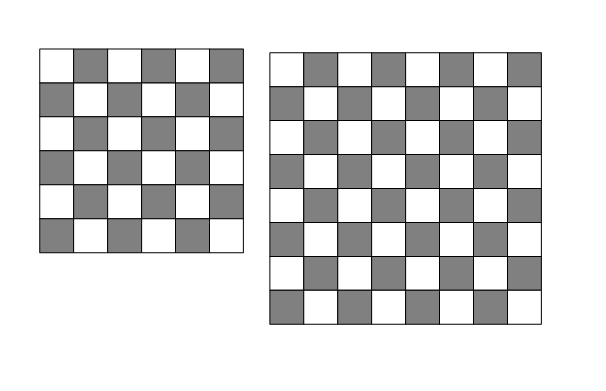
\includegraphics[width=0.8\linewidth]{001.png}
	\end{figure}
	
	组成棋盘的小格子是同样大小的正方形,黑白间错排列。
	
	现在需要一个10x10的大棋盘,希望能通过锯开这两个棋盘,重新组合出大棋盘。
	
	要求:
	
	1. 拼好的大棋盘仍然保持黑白格间错的特性。
	
	2. 两个已有的棋盘都只允许锯一锯(即锯开为两块),必须沿着小格的边沿,可以折线锯开。
	
	3。 要尽量保证8x8棋盘的完整,也就是说,从它上边锯下的那块的面积要尽可能小。
	
	要求提交的数据是:4块锯好的部分的面积。按从小到大排列,用空格分开。(约定每个小格的面积为1)
	
	比如:10 10 26 54,当然,这个不是正确答案。
	
	请严格按要求格式提交数据,不要填写任何多余的内容(比如,说明解释等)
	
	\subsection{打靶(25分)}
	
	小明参加$X$星球的打靶比赛。
	比赛使用电子感应计分系统。其中有一局,小明得了96分。
	
	这局小明共打了6发子弹,没有脱靶。
	但望远镜看过去,只有3个弹孔。
	显然,有些子弹准确地穿过了前边的弹孔。
	
	不同环数得分是这样设置的:
	1,2,3,5,10,20,25,50
	
	那么小明的6发子弹得分都是多少呢?有哪些可能情况呢?
	
	下面的程序解决了这个问题。
	仔细阅读分析代码,填写划线部分缺失的内容。
	
	\begin{lstlisting}
#include <stdio.h>
#define N 8
	
void f(int ta[], int da[], int k, int ho, int bu, int sc) {
	int i,j;
	if(ho<0 || bu<0 || sc<0) return;
	if(k==N){
		if(ho>0 || bu>0 || sc>0) return;
		for(i=0; i<N; i++){
			for(j=0; j<da[i]; j++) 
				printf("%d ", ta[i]);
		}
		printf("\n");
		return;
	}
	for(i=0; i<=bu; i++){
		da[k] = i;
		// 填空位置
		f(ta, da, k+1, _____________ , bu-i, sc-ta[k]*i);
	}	
	da[k] = 0;
}
	
int main(){
	int ta[] = {1,2,3,5,10,20,25,50};
	int da[N];
	f(ta, da, 0, 3, 6, 96);
	return 0;
}
	\end{lstlisting}
	
	
	注意:只填写划线处缺少的内容,不要填写已有的代码或符号,也不要填写任何解释说明文字等。
	
	
	\subsection{路径之谜(41分)}
	
	小明冒充$X$星球的骑士,进入了一个奇怪的城堡。城堡里边什么都没有,只有方形石头铺成的地面。
	
	假设城堡地面是$n\times n$个方格,如图所示:
	
	\begin{figure}[H]
		\centering
		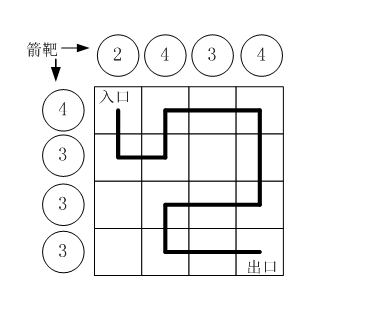
\includegraphics[width=0.8\linewidth]{002.png}
	\end{figure}
	
	按习俗,骑士要从西北角走到东南角。可以横向或纵向移动,但不能斜着走,也不能跳跃。每走到一个新方格,就要向正北方和正西方各射一箭。(城堡的西墙和北墙内各有 $n$ 个靶子)
	
	同一个方格只允许经过一次。但不必走完所有的方格。
	
	如果只给出靶子上箭的数目,你能推断出骑士的行走路线吗?
	
	有时是可以的,比如图中的例子。
	
	本题的要求就是已知箭靶数字,求骑士的行走路径(测试数据保证路径唯一)
	
	【输入】
	
	第一行一个整数$N(0<N<20)$,表示地面有 $N\times N$ 个方格
	
	第二行$N$个整数,空格分开,表示北边的箭靶上的数字(自西向东)
	
	第三行$N$个整数,空格分开,表示西边的箭靶上的数字(自北向南)
	
	【输出】一行若干个整数,表示骑士路径。
	
	为了方便表示,我们约定每个小格子用一个数字代表,从西北角开始编号: 0,1,2,3....
	比如,图中的方块编号为:
	
	0  1  2  3
	
	4  5  6  7
	
	8  9  10 11
	
	12 13 14 15
	
	示例,用户输入:
	
	4
	
	2 4 3 4
	
	4 3 3 3
	
	程序应该输出:
	
	0 4 5 1 2 3 7 11 10 9 13 14 15
	
	
	资源约定:峰值内存消耗 < 256M,CPU消耗  < 1000ms
	
	\subsection{碱基(75分)}
	
	生物学家正在对$n$个物种进行研究。其中第$i$个物种的DNA序列为$s[i]$,其中的第$j$个碱基为$s[i][j]$,碱基一定是A、T、G、C之一。
	
	生物学家想找到这些生物中一部分生物的一些共性,他们现在关注那些至少在$m$个生物中出现的长度为$k$的连续碱基序列。准确的说,科学家关心的序列用$2m$元组$(i_1,p_1,i_2,p_2,...,i_m,p_m)$表示,满足:$1\leq i_1<i_2<...<i_m\leq n$;
	且对于所有$q(0\leq q<k), s[i_1][p_1+q]=s[i_2][p_2+q]=....=s[i_m][p_m+q]$。
	
	现在给定所有生物的DNA序列,请告诉科学家有多少的2m元组是需要关注的。如果两个$2m$元组有任何一个位置不同,则认为是不同的元组。
	
	【输入格式】
	
	输入的第一行包含三个整数$n,m,k$,两个整数之间用一个空格分隔,意义如题目所述。
	
	接下来$n$行,每行一个字符串表示一种生物的DNA序列。
	
	DNA序列从$1$至$n$编号,每个序列中的碱基从1开始依次编号,不同的生物的DNA序列长度可能不同。
	
	【输出格式】
	输出一个整数,表示关注的元组个数。
	答案可能很大,你需要输出答案除以1000000007的余数。
	
	【样例输入】
	
	3 2 2
	
	ATC
	
	TCG
	
	ACG
	
	【样例输出】
	2
	
	再例如:
	【样例输入】
	
	4 3 3
	
	AAA
	
	AAAA
	
	AAA
	
	AAA
	
	【样例输出】
	7
	
	
	【数据规模与约定】对于20\%的数据,$k\leq5$,所有字符串总长$L$满足$L\leq100$;对于30\%的数据,$L\leq10000$;对于60\%的数据,$L\leq30000$;对于100\%的数据,$n\leq5,m\leq5,1\leq k\leq L\leq100000$
	
	保证所有DNA序列不为空且只会包含’A’ ’G’ ’C’ ’T’四种字母
	
	资源约定:峰值内存消耗 < 256M,CPU消耗  < 1000ms
	
	\subsection{圆圈舞(99分)}
	
	春天温暖的阳光照耀着大地,正是草原上的小动物们最快乐的时候。小动物们在草原上开了一个舞会,欢度这美好的时光。
	
	舞会上最重要的一个环节就是跳圆舞曲,$n$只小动物手拉手围成一大圈,随着音乐跳起来。在跳的过程中,小动物们可能会变换队形。它们的变换方式是动物$A$松开自己右手,动物$B$松开自己的左手,动物$A$和$B$手拉到一起,而它们对应的松开的手(如果有的话)也拉到一起。
	
	例如,假设有10只小动物,按顺序围成一圈,动物1的右手拉着动物2的左手,动物2的右手拉着动物3的左手,依次类推,最后动物10的右手拉着动物1的左手。如果通过动物2和8变换队形,则动物2的右手拉着动物8的左手,而对应的动物3的左手拉着动物7的右手,这样形成了1-2-8-9-10和3-4-5-6-7两个圈。如果此时通过动物2和6变换队形,则将形成1-2-6-7-3-4-5-8-9-10一个大圈。注意,如果此时通过动物1和2变换队形,那么队形不会改变,因为动物1的右手和动物2的左手松开后又拉到一起了。
	
	在跳舞的过程中,每个动物$i$都有一个欢乐值$H_i$和一个感动值$F_i$。
	如果两个动物在一个圈中,欢乐值会彼此影响,产生欢乐能量。如果两个动物$i, j(i\neq j)$在同一个大小为$t$的圈中,而动物$i$在动物$j$右手的第$p$个位置(动物$j$右手的第1个位置就是动物$j$右手所拉着的动物,而第2个位置就是右手第1个位置的动物右手拉着的动物,依次类推),则产生的欢乐能量为$(t-p)*H_j*F_i$。在跳舞的过程中,动物们的欢乐值和感动值有可能发生变化。
	
	圆舞曲开始的时候,所有的动物按编号顺序围成一个圈,动物$n$右手的第$i$个位置正好是动物$i$。现在已知小动物们变换队形的过程和欢乐值、感动值变化的过程,求每次变换后所有动物所产生的欢迎能量之和。
	
	【输入格式】
	
	输入的第一行包含一个整数$n$,表示动物的数量。
	
	接下来$n$行,每行两个用空格分隔的整数$H_i, F_i$,按编号顺序给出每只动物的欢乐值和感动值。
	
	接下来一行包含一个整数$m$,表示队形、欢乐值、感动值的变化次数。
	
	接下来$m$行,每行三个用空格分隔的整数$k, p, q$,当$k=1$时,表示小动物们通过动物$p$和动物$q$变换了队形,当$k=2$时,表示动物$p$的欢乐值变为$q$,当$k=3$时,表示动物$p$的感动值变为了$q$。
	
	【输出格式】
	输出$m$行,每行一个整数,表示每次变化后所有动物产生的能量之和。
	答案可能很大,你需要计算答案除以1000000007的余数。
	
	【样例输入】
	
	10
	
	1 1
	
	1 1
	
	1 1
	
	1 1
	
	1 1
	
	1 1
	
	1 1
	
	1 1
	
	1 1
	
	1 1
	
	9
	
	1 2 8
	
	1 2 6
	
	2 8 10
	
	3 5 10
	
	1 1 2
	
	1 2 1
	
	2 5 5
	
	1 4 8
	
	1 4 5
	
	【样例输出】
	
	100
	
	450
	
	855
	
	1341
	
	1341
	
	811
	
	923
	
	338
	
	923
	
	【数据规模与约定】
	对于20\%的数据,$2<=n,m<=100$。
	
	对于30\%的数据,$2\leq n,m\leq1000$。
	
	另有20\%的数据,只有$k=1$的操作且$H_i,F_i$均为1。
	
	另有20\%的数据,只有$k=1$或2的操作且$F_i$均为1。
	
	对于100\%的数据,$2<=n,m<=100000$,$0<=H_i,F_i<=10^9$,$1<=k<=3$,$k=1$时$1<=p,q<=n$且$p\neq q$,$k=2$或3时$1<=p<=n$且$0<=q<=10^9$。
	
	资源约定:峰值内存消耗 < 256M,CPU消耗  < 2500ms
	
	\section{2015 C/C++ A组}	
	
	\subsection{方格填数(19分)}
	
	在2行5列的格子中填入1到10的数字。
	要求:
	相邻的格子中的数,右边的大于左边的,下边的大于上边的。
	
	如图所示的2种,就是合格的填法。
	
	\begin{figure}[H]
		\centering
		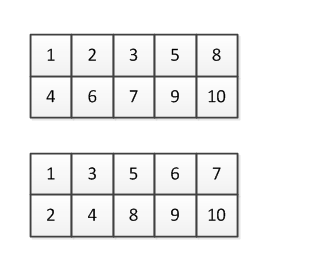
\includegraphics[width=.8\linewidth]{003.png}
	\end{figure}
	
	请你计算一共有多少种可能的方案。
	
	请提交该整数,不要填写任何多余的内容(例如:说明性文字)。
	
	\subsection{四阶幻方(35分)}
	
	把1$\sim$16的数字填入4x4的方格中,使得行、列以及两个对角线的和都相等,满足这样的特征时称为:四阶幻方。
	
	四阶幻方可能有很多方案。如果固定左上角为1,请计算一共有多少种方案。
	
	比如:
	
	1  2 15 16
	
	12 14  3  5
	
	13  7 10  4
	
	8 11  6  9
	
	以及:
	
	1 12 13  8
	
	2 14  7 11
	
	15  3 10  6
	
	16  5  4  9
	
	就可以算为两种不同的方案。
	
	请提交左上角固定为1时的所有方案数字,不要填写任何多余内容或说明文字。
	
	\subsection{显示二叉树(31分)}
	
	排序二叉树的特征是:
	某个节点的左子树的所有节点值都不大于本节点值。
	某个节点的右子树的所有节点值都不小于本节点值。
	
	为了能形象地观察二叉树的建立过程,小明写了一段程序来显示出二叉树的结构来。
	
	\begin{lstlisting}
#include <stdio.h>
#include <string.h>
#define N 1000
#define HEIGHT 100
#define WIDTH 1000
	
struct BiTree {
	int v;
	struct BiTree* l;
	struct BiTree* r;
};
	
int max(int a, int b) {
	return a>b? a : b;
}
	
struct BiTree* init(struct BiTree* p, int v) {
	p->l = NULL;
	p->r = NULL;
	p->v = v;
	return p;
}
	
void add(struct BiTree* me, struct BiTree* the) {
	if(the->v < me->v){
		if(me->l==NULL) me->l = the;
		else add(me->l, the);
	}
	else{
		if(me->r==NULL) me->r = the;
		else add(me->r, the);
	}
}
	
//获得子树的显示高度	
int getHeight(struct BiTree* me) {
	int h = 2;
	int hl = me->l==NULL? 0 : getHeight(me->l);
	int hr = me->r==NULL? 0 : getHeight(me->r);
	return h + max(hl,hr);
}
	
//获得子树的显示宽度	
int getWidth(struct BiTree* me) {
	char buf[100];
	sprintf(buf,"%d",me->v); 
	int w = strlen(buf);
	if(me->l) w += getWidth(me->l);
	if(me->r) w += getWidth(me->r);
	return w;
}
	
int getRootPos(struct BiTree* me,int x){
	return me->l==NULL? x : x + getWidth(me->l);
}
	
//把缓冲区当二维画布用 
void printInBuf(struct BiTree* me, char buf[][WIDTH], int x, int y) {
	int p1,p2,p3,i;
	char sv[100];
	sprintf(sv, "%d", me->v);
	
	p1 = me->l==NULL? x : getRootPos(me->l, x);
	p2 = getRootPos(me, x);
	p3 = me->r==NULL? p2 : getRootPos(me->r, p2+strlen(sv));
	
	buf[y][p2] = '|';
	for(i = p1; i <= p3; i++)
		buf[y+1][i] = '-';
	for(i = 0; i < strlen(sv); i++)
		buf[y + 1][p2 + i] = sv[i];
	if(p1 < p2) buf[y+1][p1] = '/';
	if(p3 > p2) buf[y+1][p3] = '\\';
		
	if(me -> l)
		printInBuf(me->l,buf,x,y+2);
	if(me -> r)
		__________________;  //填空位置
}
	
void showBuf(char x[][WIDTH]) {
	int i, j;
	for(i = 0; i < HEIGHT; i++){
		for(j = WIDTH - 1; j >= 0; j--){
			if(x[i][j] == ' ')
				x[i][j] = '\0';
			else break;
		}
		if(x[i][0])	printf("%s\n",x[i]);
		else break;
	}
}
	
void show(struct BiTree* me){
	char buf[HEIGHT][WIDTH];
	int i, j;
	for(i = 0; i < HEIGHT; i++)
		for(j = 0; j < WIDTH; j++)
			buf[i][j] = ' ';
		
	printInBuf(me, buf, 0, 0);
	showBuf(buf);
}
	
int main() {	
	struct BiTree buf[N];	//存储节点数据 
	int n = 0;              //节点个数 
	 //初始化第一个节点 
	init(&buf[0], 500); n++; 
	 //新的节点加入树中 
	add(&buf[0], init(&buf[n++],200)); 
	add(&buf[0], init(&buf[n++],509));
	add(&buf[0], init(&buf[n++],100));
	add(&buf[0], init(&buf[n++],250));
	add(&buf[0], init(&buf[n++],507));
	add(&buf[0], init(&buf[n++],600));
	add(&buf[0], init(&buf[n++],650));
	add(&buf[0], init(&buf[n++],450));
	add(&buf[0], init(&buf[n++],440));
	add(&buf[0], init(&buf[n++],220));
	
	show(&buf[0]);	
	return 0;	
}
	\end{lstlisting}
	
	对于上边的测试数据,应该显示出:

	\begin{figure}[H]
		\centering
		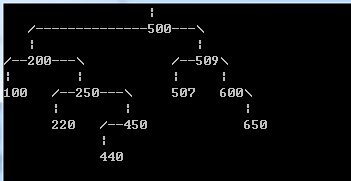
\includegraphics[width=\linewidth]{004.png}
	\end{figure}
	
	请分析程序逻辑,填写划线部分缺失的代码。	
	注意,只填写缺少的部分,不要填写已有的代码或符号,也不要加任何说明文字。
	
	\subsection{穿越雷区(41分)}
	
	$X$星的坦克战车很奇怪,它必须交替地穿越正能量辐射区和负能量辐射区才能保持正常运转,否则将报废。
	某坦克需要从$A$区到$B$区去($A$,$B$区本身是安全区,没有正能量或负能量特征),怎样走才能路径最短?
	
	已知的地图是一个方阵,上面用字母标出了$A$,$B$区,其它区都标了正号或负号分别表示正负能量辐射区。
	例如:
	\begin{lstlisting}
A + - + -
- + - - +
- + + + -
+ - + - +
B + - + -	
	\end{lstlisting}	
	
	坦克车只能水平或垂直方向上移动到相邻的区。
	
	数据格式要求:
	
	输入第一行是一个整数$n$,表示方阵的大小, $4<=n<100$
	
	接下来是$n$行,每行有$n$个数据,可能是$A$,$B$,$+$,$-$中的某一个,中间用空格分开。$A$,$B$都只出现一次。
	
	要求输出一个整数,表示坦克从$A$区到$B$区的最少移动步数。
	
	如果没有方案,则输出$-1$
	
	例如:
	用户输入:
	\begin{lstlisting}
5
A + - + -
- + - - +
- + + + -
+ - + - +
B + - + -
	\end{lstlisting}
	
	则程序应该输出:
	10
	
	资源约定:峰值内存消耗 < 512M,	CPU消耗  < 1000ms
	
	\subsection{切开字符串(75分)}
	
	Pear有一个字符串,不过他希望把它切成两段。
	这是一个长度为$N(<=10^5)$的字符串。
	Pear希望选择一个位置,把字符串不重复不遗漏地切成两段,长度分别是$t$和$N-t$(这两段都必须非空)。
	
	Pear用如下方式评估切割的方案:
	定义“正回文子串”为长度为奇数的回文子串。
	
	设切成的两段字符串中,前一段中有$A$个不相同的正回文子串,后一段中有$B$个不相同的非正回文子串,则该方案的得分为$A*B$。
	
	注意,后一段中的$B$表示的是:“...非正回文...”,而不是:“...正回文...”。
	那么所有的切割方案中,$A*B$的最大值是多少呢?
	
	【输入数据】
	
	输入第一行一个正整数$N(<=10^5)$
	
	接下来一行一个字符串,长度为$N$。该字符串仅包含小写英文字母。
	
	【输出数据】
	一行一个正整数,表示所求的A*B的最大值。
	
	【样例输入】
	
	10
	
	bbaaabcaba
	
	【样例输出】
	38
	
	【数据范围】
	对于20\%的数据,$N<=100$;
	对于40\%的数据,$N<=1000$;
	对于100\%的数据,$N<=10^5$
	
	资源约定:峰值内存消耗 < 512M,CPU消耗  < 1000ms
	
	\subsection{铺瓷砖(99分)}
	
	为了让蓝桥杯竞赛更顺利的进行,主办方决定给竞赛的机房重新铺放瓷砖。机房可以看成一个$n*m$的矩形,而这次使用的瓷砖比较特别,有两种形状,如下图所示。在铺放瓷砖时,可以旋转。
	
	\begin{figure}[H]
		\centering
		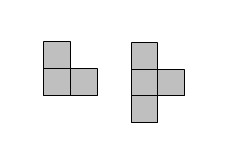
\includegraphics[width=.8\linewidth]{005.png}
	\end{figure}
	
	主办方想知道,如果使用这两种瓷砖把机房铺满,有多少种方案。
	
	【输入格式】
	输入的第一行包含两个整数,分别表示机房两个方向的长度。
	
	【输出格式】
	输出一个整数,表示可行的方案数。这个数可能很大,请输出这个数除以65521的余数。
	
	【样例输入1】
	4 4
	
	【样例输出1】
	2
	
	【样例说明1】
	这两种方案如下图所示:
	
	\begin{figure}[H]
		\centering
		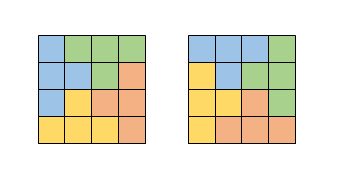
\includegraphics[width=.8\linewidth]{006.png}
	\end{figure}
	
	【样例输入2】
	2 6
	
	【样例输出2】
	4
	
	【数据规模与约定】
	对于20\%的数据,$1<=n, m<=5$。
	对于50\%的数据,$1<=n<=100,1<=m<=5$。
	对于100\%的数据,$1<=n<=10^{15},1<=m<=6$。
	
	资源约定:峰值内存消耗 < 512M,CPU消耗  < 5000ms
	
\end{document}

